\input /Users/davidmcallester/ICloude/tex/SlidePreamble
\input /Users/davidmcallester/ICloude/tex/preamble


\begin{document}

{\Huge
  \centerline{\bf TTIC 31230,  Fundamentals of Deep Learning}
  \vfill
  \centerline{David McAllester, Autumn   2021}
  \vfill
  \centerline{\bf Mutual Information Coding}
  \vfill
  \vfill

\slideplain{Mutual Information Coding}
\centerline{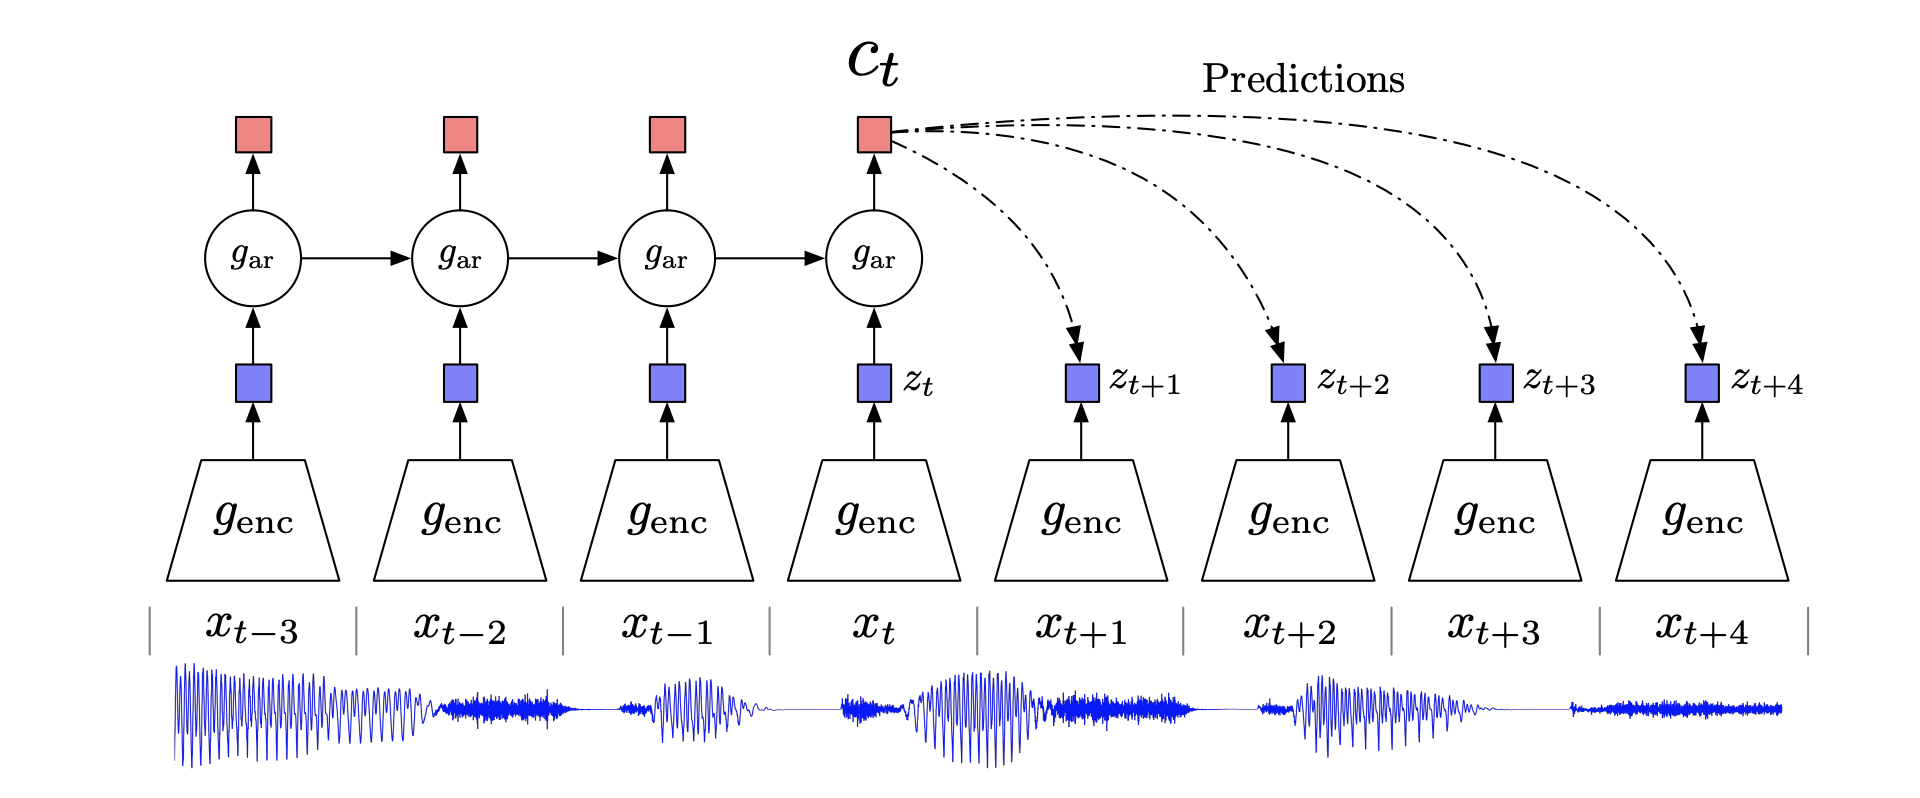
\includegraphics[width = 6 in]{\images/CPC}}
\centerline{\huge van den ORD et al. 2018}

\vfill
We want to find codes that maximize the mutual information between the codes for different but related inputs.  In the figure we want the codes to maximize the mutual information between $C_t$ and $z_{t+k}$.


\slide{wav2vec 2.0}

Mutual information coding as pretraining of speech features.

\vfill
Trained on 53k hours of unlabeled audio (no text) they convert speech to a sequence of discrete quantized vectors they call ``pseudo-text units''.

\vfill
Using the pre-trained transcription of speech sound into pseud-text they achieve the previous state of the art for training on 100 hours of transcriped text but using only one hour instead of 100 hours.

\vfill
\centerline{\huge Baevski et al., 2020}

\slide{SimCLR, BYOL and SwAV}

Mutual information coding as pretraining of image features.

\centerline{\includegraphics[width = 4.0in]{\images/BYOL}\hfill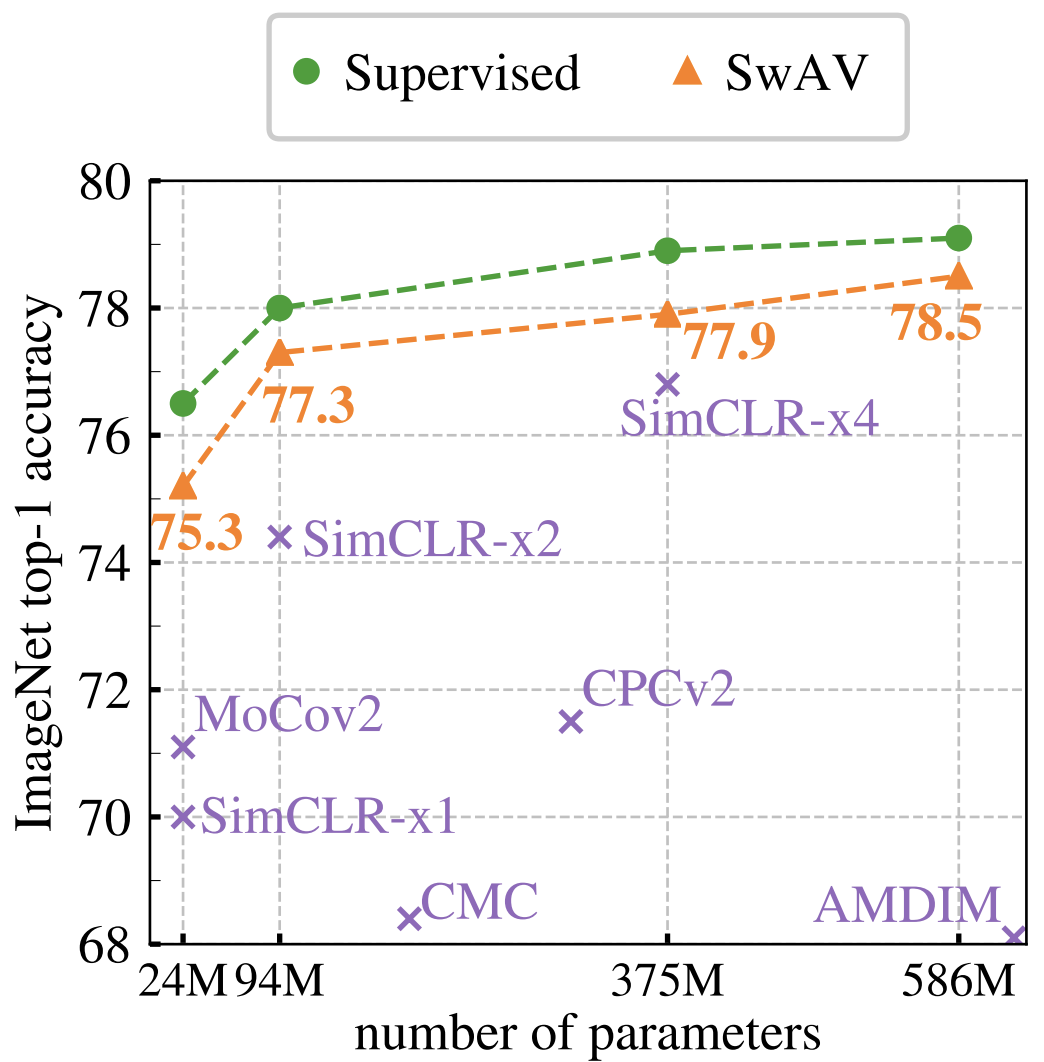
\includegraphics[width = 4.0in]{\images/SwAV}}

\slide{Mutual Information Coding}

Consider a population distribution on pairs $\tuple{x,y}$.

\vfill
For example $x$ might be an image and $y$ a sound wave.

\vfill
We are interested in extracting latent variables $z_x$ and $z_y$ from $x$ and $y$ respectively.

\vfill
For example $z_x$ might be a bag of words extracted from the image and $z_y$ a bag of words extracted from the sound wave.


\slide{Mutual Information Coding}

For a population on $\tuple{x,y}$ we introduce two discrete latent variables $z_x$ and $z_y$ defined by
models {\color{red} $P_\Phi(z_x|x)$} and {\color{red} $P_\Phi(z_y|y)$}.

\vfill
$$\Phi^* = \argmax_{\Phi} \; I_{\pop,\Phi}(z_x,z_y) - \beta (H_{\pop,\Phi}(z_x) + H_{\pop,\Phi}(z_y))$$

\vfill
Here we are asking to maximize the mutual information while (intuitively) limiting the information in $z_x$ and $z_y$.

\vfill
In the bag of words example we are asking to maximize the mutual information between the two probability distributions on bags of words while limiting the information in the bags.

\slide{Mutual Information Coding}

$$\Phi^* = \argmax_{\Phi} \; I_{\pop,\Phi}(z_x,z_y) - \beta (H_{\pop,\Phi}(z_x) + H_{\pop,\Phi}(z_y))$$

\vfill
Limiting the information in $z_x$ and $z_y$ prevents the trivial solution of $z_x = x$ and $z_y = y$.

\vfill
{\bf Here we only model distributions on $z_x$ and $z_y$.  Unlike GANs and VAEs, there is no attempt to model distributions on the observables $x$ and $y$.}

\slide{Mutual Information Coding}

\begin{eqnarray*}
\Phi^* & = & \argmax_{\Phi} \; I_{\pop,\Phi}(z_x,z_y) - \beta (H_{\pop,\Phi}(z_x))) \\
\\
 & = & \argmax_{\Phi} \; (1-\beta)H_{\pop,\Phi}(z_x) -\; H_{\pop,\Phi}(z_x|z_y) \\
 \\
 & = & \argmin_\Phi\;H_{\pop,\Phi}(z_x|z_y) - (1-\beta)H_{\pop,\Phi}(z_x)
\end{eqnarray*}

\slide{Mutual Information Coding}

We can estimate entropies by cross-entropies

\begin{eqnarray*}
\Phi^* & = & \argmin_\Phi\;H_{\pop,\Phi}(z_x|z_y) - (1-\beta)H_{\pop,\Phi}(z_x) \\
\\
& \leq & \argmin_\Phi\;\hat{H}_{\pop,\Phi,\Psi}(z_x|z_y) - (1-\beta)H_{\pop,\Phi}(z_x) \\
\\
& \approx\mathrm{?} & \argmin_\Phi\;\hat{H}_{\pop,\Phi,\Psi}(z_x|z_y) - (1-\beta)\hat{H}_{\pop,\Phi,\Theta}(z_x) \\
\end{eqnarray*}

Here the cross-entropy models $\Psi$ ans $\Theta$ are adversarial.

\slide{Contrastive Predictive Coding}

$$\Phi^* = \argmax_{\Phi} \; I_{\pop,\Phi}(z_x,z_y)$$

\vfill
It turns out that we can give a lower bound on the mutual information term using {\bf noise contrastive estimation}.

\slide{A Contrastive Lower Bound}

We now give a contrastive lower bound for general mutual information $I(z,w)$ given only the ability to sample from the joint distribution on $z$ and $w$.

\vfill
For $N \geq 2$ let {\color{red} $c_{z,w}$} be the density defined by drawing pairs $(z_1,w_1), \ldots (z_n,w_n)$ from the population
and then constructing the tuple $(i,z_1,\ldots,z_N,w_i)$ where $i$ is drawn uniformly from $1$ to $N$.

\slide{A Constrastive Bound}
We train the codes to so that we can predict $i$ from $(z_1,\ldots,z_n,w)$.
{\huge
\begin{eqnarray*}
\Phi^* & = & \argmin_\Phi \;E_{(i,z_1\ldots,z_N,w) \sim c_{z,w}}\;-\ln P_\Phi(i|z_1,\ldots,z_n,w) \\
\\
& = & \argmin_\Phi\;{\cal L}(\Phi) \\
\\
P_\Phi(i|z_1,\ldots z_n,w) & = & \softmax_i\;s_\Phi(z_i,w) \;\;\;\mbox{(required)} \\
\\
I(z,w) & \geq & \ln N - {\cal L}(\Phi)
\end{eqnarray*}
}

See Chen et al., On Variational Bounds of Mutual Information, May 2019.

\slide{Forcing $z_x$ and $z_y$ to be Useful}

In the objective

$$\Phi^* = \argmax_{\Phi} \; I_{\pop,\Phi}(z_x,z_y) - \beta ({\color{red} H_{\pop,\Phi}(z_x)} + {\color{red} H_{\pop,\Phi}(z_y)})$$


the limitation on the entropy of $z_x$ and $z_y$ block the trivial solution of $z_x = x$ and $z_y = y$.


\vfill
CPC applications have used an alternative.

\slide{Forcing $z_x$ and $z_y$ to be Useful}

\begin{eqnarray*}
\Phi^* & = & \argmin_\Phi \;E_{(i,z_x^1\ldots,z_x^n,z_y) \sim c_{z_x,z_y}}\;-\ln P_\Phi(i|z_x^1,\ldots,z_x^n,z_y)
\end{eqnarray*}

\begin{eqnarray*}
P_\Phi(i|z_x^1,\ldots,z_x^n,z_y) & = & \softmax_i\;{\color{red} z_y^\top z_x^i}
\end{eqnarray*}


\vfill
Requiring that the score be a simple inner product blocks $z_x = x$ and $z_y = y$ and forces
$z_x$ and $z_y$ to carry the information in a linearly extractible way.

\slide{Contrastive Predictive Coding for Speech}

wav2vec uses contrastive predictive coding (CPC)

\centerline{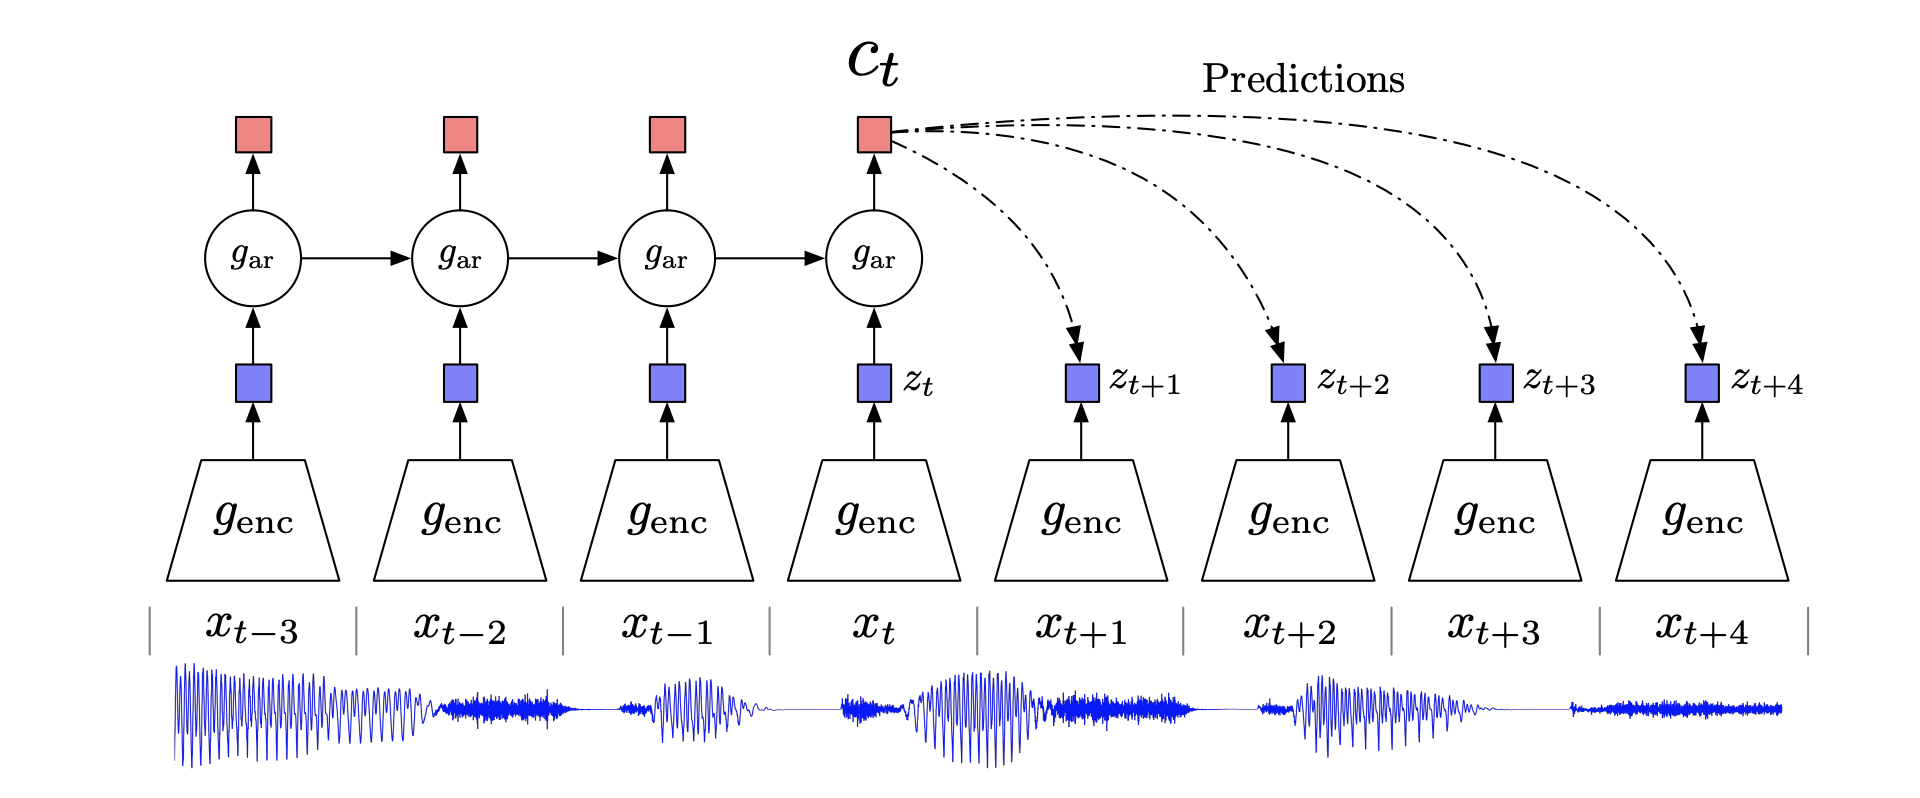
\includegraphics[width = 5 in]{\images/CPC}}

\slide{Contrastive Predictive Coding for Images}

(SimCLR:) A Simple Framework for Contrastive Learning of Visual Representations, Chen et al., Feb. 2020 (self-supervised leader as of February, 2020).

\vfill
They construct a distribution on pairs $\tuple{x,y}$ defined by drawing an image from ImageNet and then drawing $x$ and $y$ as random ``augmentations'' (modifications) of the image.

\vfill
The training maximizes the contrastive lower bound on $I(x,y)$.

\slide{Contrastive Predictive Coding for Images}

A resulting feature map $z_\Phi$ on images is extracted from this training.

\vfill
The feature map $z_\Phi$ is tested by using a {\color{red} linear} classifier for ImageNet based on these features.

\slide{SimCLR}

\centerline{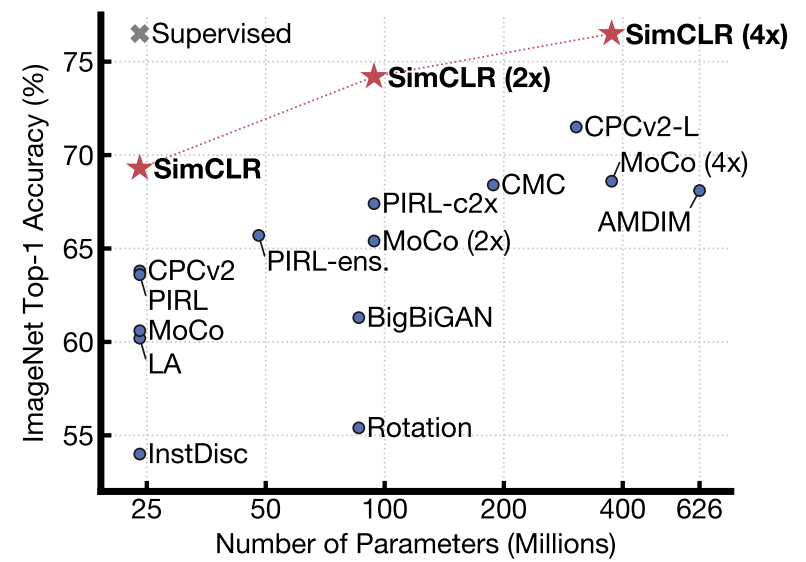
\includegraphics[height=4.5 in]{\images/SimCLR}}
\centerline{\huge Chen et al. 2020}

\slide{BYOL and SwAV do not use CPC}

BYOL and SwAV train only on cross-entropy conditional probability

$${\cal L}(\Psi) = -\ln P_\Psi(z_x|z_y)$$

This has a degenerate solution where the code for $z_x$ is constant independent of $x$.  Complex hacks are used to cause this not to happen
but performance is improved over the contrastive SimCLR.

\slide{BOYL and SwAV}

\centerline{\includegraphics[width = 4.0in]{\images/BYOL}\hfill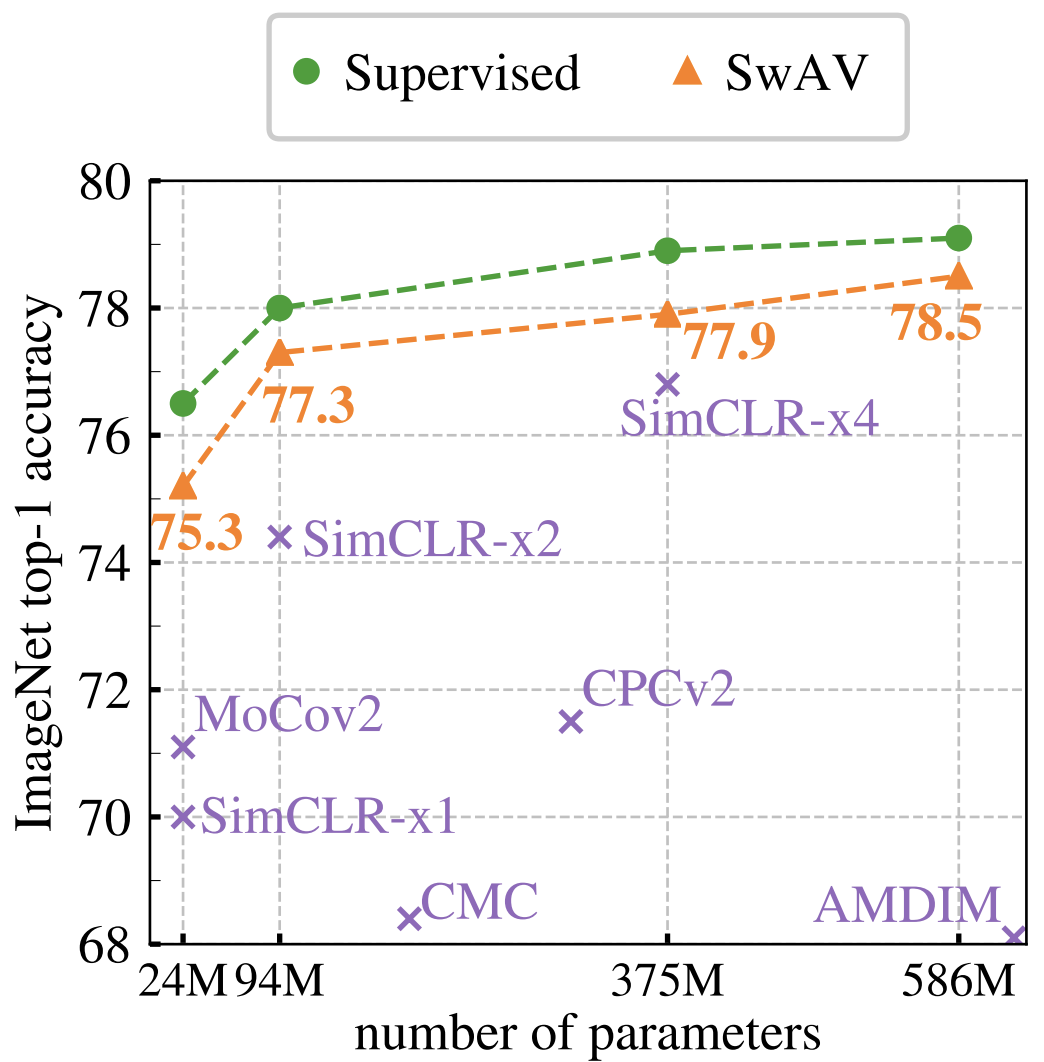
\includegraphics[width = 4.0in]{\images/SwAV}}

\centerline{\huge Grill et al. 2020, Caron et al. 2021}

\slide{END}

}
\end{document}


\slide{END}

}
\end{document}

